\documentclass[a4paper, adobefonts]{ctexart}

\usepackage[top=1.2in, bottom=1.2in, left=1in, right=1in]{geometry}
\usepackage{minted, graphicx, hyperref}

\hypersetup{colorlinks=true, linkcolor=blue}

\title{操作系统实验报告7}
\author{蔡日骏\quad12348003}

\begin{document}
\maketitle

\section{简介}
本次实验扩充了上次实验的AssignmentOS内核,实现了\verb|fork|、\verb|wait|和\verb|_exit|
系统调用。系统调用的ABI使用旧版本Linux风格的\verb|0x80|中断实现方式。在实现\verb|fork|
系统调用时,通过虚拟内存和物理内存页引用计数方式实现Copy-on-write机制。

\section{实现}

通过中断实现系统调用比较简单,在中断描述符表\verb|0x80|处写入系统调用调度器,调度器读取
通用寄存器的值,查询系统调用映射表,调用相应的系统调用处理函数即可。系统调用调度器的实现
如下:

\begin{minted}{c}
typedef int (*syscall_t)(int, int, int);  /* 系统调用处理函数指针类型 */

/* 系统调用映射表 */
const syscall_t SYSCALL_TABLE[] = {
    NULL,
    sys_exit,
    sys_fork,
    NULL,
    NULL,
    NULL,
    NULL,
    sys_wait
};

/* 系统调用调度器 */
int _syscalls()
{
    register int32_t syscall_num asm("eax"),
             p1 asm("ebx"),
             p2 asm("ecx"),
             p3 asm("edx");
    return SYSCALL_TABLE[syscall_num](p1, p2, p3);
}
\end{minted}

下面分别针对本次实验中实现的3个系统调用进行详细介绍。

\subsection{\_exit}
\verb|_exit|系统调用用于以一个退出码结束一个进程。该系统调用需要完成的工作为把当前进程
的状态设置为\verb|ZOMBIE|、设置进程退出码、释放进程用户空间的内存页、尝试唤醒等待中的
父进程。

\begin{minted}{c}
int sys_exit(int code, int _1, int _2)
{
    struct Task_t *p_task = task_list[CURRENT_TASK->ppid];
    CURRENT_TASK->exit_code = code;                 /* 设置进程退出码 */
    CURRENT_TASK->status = ZOMBIE;                  /* 设置进程状态 */
    free_page_structure(CURRENT_TASK->page_dir);    /* 释放用户空间内存页 */
    if(p_task && p_task->status == BLOCKED && p_task->block_event == WAIT_CHILD)
        wake_up_pid(p_task->pid);                   /* 尝试唤醒父进程 */
    CURRENT_TASK = NULL;
    TASK_SWITCH();                                  /* 释放控制权进行任务切换 */
}
\end{minted}

进程退出时,并不需要释放自己的进程控制数据结构,也不会释放全局描述符表中的对应项。这些
结构的清理工作将由父进程完成。

\subsection{wait}
AssignmentOS的\verb|wait|系统调用跟POSIX标准的\verb|wait|系统调用有所不同。POSIX的\verb|wait|
等待任意一个子进程退出,AssignmentOS的\verb|wait|等待指定的一个子进程退出,相当于一个简化版的
POSIX中的\verb|waitpid|。

父进程在等待某个子进程的过程中可能会其他退出的子进程被唤醒,因此每次\verb|pwait|函数返回时都
需要判断刚刚退出的是不是正在等待的子进程。

当子进程退出后,父进程需要清理子进程的进程控制数据结构,并释放全局描述符表中对应的项。

\begin{minted}{c}
int sys_wait(int pid, int _1, int _2)
{
    struct Task_t *c_task = task_list[pid];
    if(c_task == NULL)
        return -1;
    while(c_task->status != ZOMBIE) {               /* 检查等待的子进程状态 */
        CURRENT_TASK->block_event = WAIT_CHILD;     /* 设置当前进程状态为阻塞 */
        pwait();                                    /* 阻塞当前进程,进程任务切换 */
    }
    GDT[pid].present = 0;                           /* 释放GDT中对应的项 */
    task_list[pid] = NULL;                          /* 清除任务指针列表中的项 */
    dec_page_ref(PT_NUM_ADDR(c_task));              /* 释放PCB */
    return c_task->exit_code;                       /* 返回子进程的退出码 */
}
\end{minted}

\subsection{fork}
由于分页机制和需要实现Copy-on-write,\verb|fork|系统调用的实现有点麻烦。

除了复制基本的进程控制结构,还需要复制页目录表/页表。此外,实现Copy-on-write需要处理
\verb|0x0E|中断(Page fault),而该中断需要在内核态栈上写入数据,因此内核态栈不能实现
Copy-on-write,所以需要在\verb|fork|时复制内核态栈。

在复制页表时,同时需要增加对应物理内存页的引用计数,并把两个进程的页表中对应项的写保护
打开。处理Page fault时,需要检查对应物理内存页的引用计数。如果为1,则直接关闭写保护即可。
否则,需要复制该页,减少引用计数,并关闭写保护。

\verb|fork|系统调用需要保存当前的上下文而不是上次任务切换时的上下文,因此使用下面的汇编
函数作为系统调用处理函数,把寄存器的值传递给真正创建子进程的C函数。

\begin{minted}{nasm}
extern _sys_fork
global sys_fork
sys_fork: ;not an int handler but called by an int handler
    enter 0, 0
    push gs
    push fs
    push ds
    push ss
    push cs
    push es
    push edi
    push esi
    push ebp
    push esp
    push ebx
    push edx
    push ecx
    pushfd
    push after_fork     ;子进程的EIP指针设置为进程分叉后而不是当前的值
    call _sys_fork      ;调用C函数创建子进程
after_fork:
    leave
    ret
\end{minted}

\begin{minted}{c}
uint16_t _sys_fork(uint32_t eip, uint32_t eflags, uint32_t ecx, uint32_t edx,
        uint32_t ebx, uint32_t esp, uint32_t ebp, uint32_t esi, uint32_t edi,
        uint32_t es, uint32_t cs, uint32_t ss, uint32_t ds, uint32_t fs,
        uint32_t gs)
{
    cli();

    /* 创建子进程的进程控制数据结构 */
    uint32_t task_struct_pn = alloc_phy_page(0, 1023);
    map_page(CURRENT_TASK->page_dir, task_struct_pn, task_struct_pn,
        false, false, true);
    struct Task_t *t = (struct Task_t *)(task_struct_pn << 12);
    memcpy(t, CURRENT_TASK, 1024);
    /* 复制页目录表和页表 */
    t->page_dir = clone_page_structure((uint32_t *)CURRENT_TASK->tss.cr3);
    t->tss.cr3 = (uint32_t)t->page_dir;

    /* 复制内核态堆栈 */
    uint32_t stack = alloc_phy_page(1024, max_page_num);
    map_page(CURRENT_TASK->page_dir, 1024, stack, false, false, true);
    memcpy((uint32_t *)0x400000, (uint32_t *)(0xfffff000), 4096);
    map_page(t->page_dir, 0xfffff, stack, false, true, true);

    /* 写入子进程的上下文 */
    t->tss.eip = eip;
    t->tss.eflags = eflags;
    t->tss.eax = 0;     /* 子进程的返回值为0 */
    t->tss.ecx = ecx;
    t->tss.edx = edx;
    t->tss.ebx = ebx;
    t->tss.esp = esp;
    t->tss.ebp = ebp;
    t->tss.esi = esi;
    t->tss.edi = edi;
    t->tss.es = es;
    t->tss.cs = cs;
    t->tss.ss = ss;
    t->tss.ds = ds;
    t->tss.fs = fs;
    t->tss.gs = gs;

    t->ppid = CURRENT_TASK->pid;
    add_task(t);        /* 把子进程添加到任务列表 */

    sti();
    return t->pid;      /* 父进程返回子进程的PID */
}
\end{minted}

Page fault的处理如下:

\begin{minted}{c}
void _page_fault(uint32_t addr, uint32_t errcode)
{
    bool present = errcode & 0x1, write = errcode & 0x2;
    if(present && write) {  /* copy-on-write */
        uint32_t *page_table;
        uint32_t vir_pn, phy_pn;
        vir_pn = PT_NUM_ADDR(addr);
        page_table = (uint32_t *)(CURRENT_TASK->page_dir[PD_IDX(vir_pn)]
            & 0xfffff000);
        phy_pn = page_table[PT_IDX(vir_pn)] >> 12;
        if(phy_mem_rc[phy_pn] > 1) {        /* 仍为共享状态 */
            memcpy(PAGE_CPY_TMP, (void *)addr, 4096);
            dec_page_ref(phy_pn);           /* 减少引用计数 */
            phy_pn = alloc_phy_page(1024, max_page_num);
            page_table[PT_IDX(vir_pn)] &= 0xfff;
            page_table[PT_IDX(vir_pn)] |= phy_pn << 12; /* 重定向到新物理页 */
            memcpy((void *)addr, PAGE_CPY_TMP, 4096);   /* 复制数据 */
        }
        page_table[PT_IDX(vir_pn)] |= 0x2;  /* 关闭写保护 */
    }
}
\end{minted}

\section{演示}

在终端中运行\verb|fork|命令进行上面3个系统调用的测试。该测试程序如下:

\begin{minted}{c}
void fork_test()
{
    uint16_t pid;
    char pid_str[8];
    itos(CURRENT_TASK->pid, pid_str);
    /* 输出当前进程(父进程)的PID */
    print_str("Fork test\nMy PID is ", 0xE8);
    print_str(pid_str, 0xE8);
    print_str(".\nI'm going to fork now.\n", 0xE8);

    pid = fork();   /* 进行分叉 */
    if(pid) {       /* 父进程 */
        itos(pid, pid_str);
        print_str("Fork success. I'm the parent process.\n", 0xE8);
        print_str("The PID of the child process is ", 0xE8);
        print_str(pid_str, 0xE8);   /* 输出子进程的PID */
        print_str(".\nWait for the child process to exit to prevent it"
            " from becoming a zombie.\n", 0xE8);
        wait(pid);  /* 等待子进程退出 */
        print_str("I'm the parent process and I'm exiting now. Bye!\n", 0xE8);
    } else {        /* 子进程 */
        itos(CURRENT_TASK->ppid, pid_str);
        print_str("I'm the child process.\nMy parent is ", 0x8E);
        print_str(pid_str, 0x8E);   /* 输出父进程的PID */
        print_str(".\nI'm exiting now. Bye!\n", 0x8E);
    }
    _exit(0);       /* 结束进程 */
}
\end{minted}

效果如图:

\begin{figure}[htp!]
    \center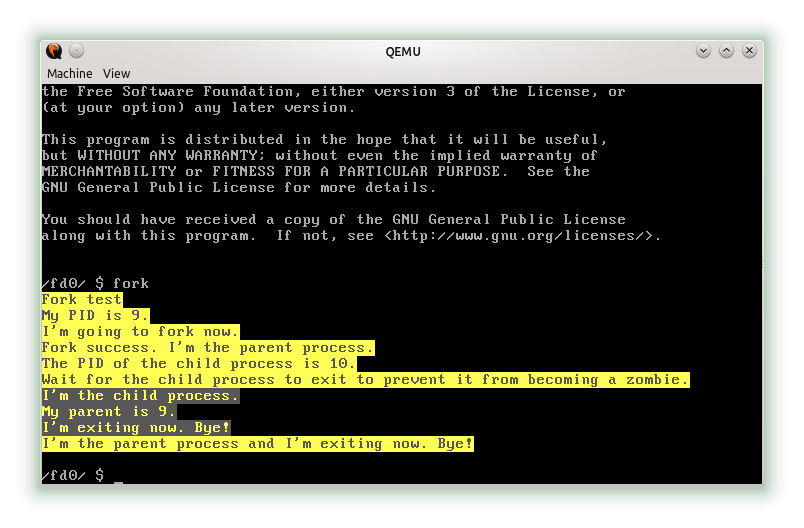
\includegraphics[scale=0.72]{fork_test.png}
\end{figure}

\end{document}
